\documentclass[a4paper,man,natbib]{apa6}
%\usepackage[square]{natbib}
\usepackage{microtype}
\usepackage{mathtools} % needed
\usepackage{hyperref}
%\usepackage{stmaryrd} % not needed
\usepackage{tabularx}
\newcolumntype{Y}{>{\raggedright\arraybackslash}X}

\usepackage[normalem]{ulem}
%\linespread{1.3}
% use apa defaults
\hypersetup{hidelinks=true}
% let's not be garish
\usepackage{lingex} % some linguistic-style example numbering


\newcommand*{\smex}[1]{\textit{#1}} % 'small example'
\newcommand*{\spex}[1]{``{#1}''} % 'spoken example'
\newcommand*{\term}[1]{\emph{#1}} % introducing a new term
\newcommand*{\citegen}[1]{\citeauthor{#1}'s~(\citeyear{#1})}
\newcommand*{\SE}{\mathit{SE}} % fix funny "SE" spacing

\title{Contextual Effects on Online Pragmatic Inferences of Deception}
\author{Josiah P.\@ J.\@ King, Jia E.\@ Loy, Martin Corley}
\affiliation{Psychology, PPLS, University of Edinburgh}
\ifapamodeman{\note{\begin{flushleft}%
Josiah King\\
Philosophy, Psychology and Language Sciences\\
University of Edinburgh\\
7~George Square\\
Edinburgh EH8~9JZ, UK\\[1ex]
\url{J.P.J.King@sms.ed.ac.uk}
\end{flushleft}}}




\shorttitle{Contextual Effects on Deception}

\abstract{Where the veracity of a statement is in question, listeners tend to interpret disfluency as signalling dishonesty.
Previous research in deception suggests that this results from a speaker model, linking lying to cognitive effort, and effort to disfluency.
However, the disfluency-lying bias occurs very quickly: 
Might listeners instead simply heuristically associate disfluency with lying?
To investigate this, we look at whether listeners' disfluency-lying biases are sensitive to context.
Participants listened to a potentially dishonest speaker describe treasure as being behind a named object, while viewing scenes comprising the referent (the named object) and a distractor. 
Their task was to click on the treasure's suspected true location. 
In line with previous work, participants clicked on the distractor more following disfluent descriptions, and this effect corresponded to an early fixation bias, demonstrating the online nature of the pragmatic judgment.
The present study, however, also manipulated the presence of an alternative, local cause of speaker disfluency: The speaker being momentarily distracted by a car-horn.
When disfluency could be attributed to speaker distraction, participants initially fixated more on the referent, only later fixating on and selecting the distractor. 
These findings support the speaker modeling view, showing that listeners can take momentary contextual causes of disfluency into account.}


\begin{document}
\maketitle


%\section{Background}
% apa style:  Don't start with section heading
\noindent
Everyday speech is for the most part spontaneous, and thus often disfluent, containing pauses, \spex{um}s, \spex{uh}s, repetitions, revisions, and mispronunciations.
Excluding silent pauses, naturally occurring speech has a rate of approximately~6 to~10 disfluencies per~100 words \citep{Bortfeld2001,FoxTree1995}.
The disfluent nature of speech is just one of many variable aspects of \emph{how} an utterance might be presented, and listeners must be able to cope with this variability in order to successfully understand a speaker.

Disfluencies in speech are not merely incidental.  
Speakers are more disfluent when utterance planning involves low-frequency words \citep{Beattie1979}, less-preferred syntactic structures \citep{Cook2009}, discourse-new expressions \citep{arnold2000heaviness}, or a greater choice of expressive alternatives \citep{Schachter1991}.
In this way, disfluencies provide paralinguistic `cues' about the content of a speaker's message.
Research has shown that listeners can, and do, exploit these cues to make predictions about upcoming speech.
For example, following a disfluency, they are more likely to predict the introduction of a new object into the discourse, as shown by visual world eye movements \citep{Arnold2004}, and less likely to have difficulty integrating an unpredictable word into its context, as indexed by a reduction in the N400~ERP component \citep{Corley2007}.

Evidence from a series of eye-tracking experiments suggests that predictions like these are sensitive to context.
\citet{Arnold2007} asked participants to click on depictions of easy-to-name (ice-cream) or harder-to-name (abstract symbol) items in response to auditory instructions.
When the instructions were disfluent, participants were more likely to fixate harder-to-name items before they heard the item name.
Importantly, these fixation biases were modulated when participants were told that the speaker had object agnosia, and hence might be presumed to have difficulty naming easy-to-name items.
The fact that a prediction that a hard-to-name item will follow a disfluency can be modulated by contextual information suggests that, on encountering a disfluency, participants are not merely making a stochastic prediction about what might be mentioned next.
Instead, they may be actively modeling the speaker in order to account for the disfluency encountered and make situation-specific predictions.

However, the picture is far less clear when the cause of the disfluency is local, in the sense that it could be assumed to be the cause of a specific instance of disfluency, rather than of a heightened probability of disfluency in general.
In \citeauthor{Arnold2007}'s Experiment~3, for example, local causes (beeps and construction noises, assumed to distract the speaker momentarily) did not affect listeners' biases to fixate harder-to-name objects following disfluency.
Moreover, several studies have shown that listeners do not seem especially sensitive to the nature of the disfluency:  They have been shown to be affected by dog barks \citep{bailey2003disfluencies} and sine waves \citep{corley2011helps} when they are substituted for filled-pause disfluencies.
This sensitivity to non-linguistic interruptions sits poorly with the idea that the listener is modeling the speaker's production system, to anything greater than a superficial extent.

One reason that it is hard to conclude what is being modeled is that, in the studies outlined above, the effects of disfluency are ephemeral.
Disfluency might affect what listeners think they are about to hear, but it has no lasting consequences at the message level:
The fluent and disfluent versions of the utterances used mean the `same thing'.
For that reason, the consequences to the listener of mismodeling the speaker are trivial, and the behavioral consequences of any such modeling relatively hard to detect.
However, a parallel literature shows that in some circumstances, disfluency has pragmatic effects, in that it has direct consequences for the way a listener interprets an utterance.
%
%FO(A)K; other pragmatics; lying; Jia \ra{}question:  Now we're talking about \emph{pragmatic} effects, is there evidence of speaker modelling?
For example, \citet{Brennan1995} based their comprehension study on evidence that speakers use disfluency to manage difficulty in retrieving information \citep{Smith1993}.
Participants were played recordings of answers to general knowledge questions which had been obtained during a production study.
The answers were digitally edited and were sometimes preceded by either a silent pause or a filler.
Listeners rated the answers as being less likely to be correct when the recorded answers were preceded by silence or fillers.
In other words, their interpretations of, rather than simply predictions concerning, the utterances they heard were directly affected by disfluency \citep[see also][]{Swerts2005}.
Listeners faced with disfluency had less confidence in the speaker's knowledge (a weaker ``Feeling of Another's Knowing'', or FOAK), and therefore revised their estimates concerning the factual correctness of what was being said.

%%% NB I couldn't find much evidence of "other pragmatic" effects.  I
%%% do seem to recall some social psych papers talking about
%%% disfluency as hedging; would be great if we could find those

As well as producing statements about which they have little confidence, speakers can easily utter propositions which they know to be false.
This form of lying is often thought to be associated with cognitive effort.
According to this view, the increased load involved in formulating and uttering a lie may lead speakers to provide verbal and non-verbal cues to deception, including disfluency \citep{Zuckerman1981,depaulo2003cues}.
Listeners' interpretations appear to reflect such a hypothesis:
\citet{Zuckerman1981} found hesitations in speech to be reliably associated with a perception of dishonesty, in both judgments made by speakers about themselves, and judgments made about another speaker.
%%%%%%%% need link here. importance is comp not produ.
%%%% DOES THIS FLOW?

In both FOAK and lying research, the proposed mechanism by which the interpretation of what is said is affected by disfluency is via \term{speaker modeling}:
By reverse inference, disfluency is a symptom of cognitive difficulty, and cognitive difficulty is the consequence of limited knowledge (FOAK) or of inventing a situation (lying).
In other words, to conclude that the speaker is lying requires reasoning about his or her cognitive state, in line with earlier claims by \citet{Arnold2007}.
However, listeners may in fact not reason in this way.
Instead, they may heuristically associate certain aspects of spoken performance with uncertainty or lying, perhaps based on previous co-occurrence, or a superficial model of the speaker.
This heuristic association would only be affected by very clear evidence that it wasn't relevant.

One reason for believing that the association between disfluency and lying is heuristically calculated is evidence from \citet{Loy2016}, which highlights the speed at which pragmatic interpretations are made.
\citeauthor{Loy2016}'s study was framed as a treasure hunting game, in which listeners were asked to guess the location of a reward by clicking on one of two depicted objects in each trial, behind which they believed the treasure to be hidden.
Participants heard recorded utterances which indicated the location of the treasure, and which were either fluent or disfluent (\spex{The treasure is behind [the]/[thee, uh] \textless referent\textgreater}).
Participants were told that the speaker would be dishonest half of the time. 
The judgments which participants made about the speaker's honesty in each trial were implicitly measured by examining which of the two objects they clicked:
Clicking on the named object corresponded to a judgment that the speaker was telling the truth, whereas a click on the other object meant that the speaker was thought to be lying.
In line with previous research linking disfluency to deception \citep{Zuckerman1981},  participants were less likely to click on the named object following disfluent utterances (and instead, tended to click on the object which had not been mentioned).
Importantly, eye- and mouse-tracking records showed that this effect emerged as soon as it became clear which of the two objects was being named:
In other words, participants' pragmatic judgments were shown to be influenced by disfluency at the earliest detectable moment.
If detailed speaker modeling is occurring, any inferences regarding the cause of a given disfluency would have to be made very fast.

%%% so this becomes another reason for assuming that it's a heuristic????
%%%%%%%%%%%%%%%%%%%%%%%%%%%%%%%%%%%%%%%%%%%%%%%%%%%%%%%%%%%%%%%%%%%%%%%%%
Another reason for assuming that a heuristic is at play is that listeners' interpretations of disfluency may be inaccurate.
Although listeners tend to associate disfluency with lying \citep{Loy2016,Zuckerman1981}, some evidence suggests that, in production, disfluency occurs more frequently during truth-telling than during deception \citep{Arciuli2010markers,Arciuli2009lies,Benus2006pauses}.
\citet{DePaulo1982actual} demonstrated a mismatch between disfluency as an actual and as a perceived cue to deception:
The rates of filled pauses produced by speakers did not differ during descriptions they made about people whom they liked or disliked from descriptions made when they were asked to pretend to feel the opposite way about them. 
However, when listening to the descriptions made by other participants, higher rates of filled pauses were associated with an interpretation that the speaker was being deceitful \citep[see also][]{loy2016lying}.


The evidence cited above suggests that, at least for the case of deception, the influence of speaker disfluency is fast, and not always accurate: 
Listeners appear to rely on a rule-of-thumb association between disfluency and lying.
However, it is possible that any inaccuracy is actually the result of a more detailed attempt to model the speaker.
Lying is associated with cognitive effort, and cognitive effort is associated with disfluency, perhaps predicated not on experience as a listener but on introspection as a speaker:
Speakers believe themselves to be more disfluent when lying \citep{Zuckerman1981}, and this belief extends to others' language production.
Evidence for this conjecture would lie in whether listeners' assessments of speaker veracity were affected by specific circumstances that a heuristic would be unlikely to take into account.
One such circumstance would be the availability of an alternative cause of a given disfluency, such as the speaker being momentarily distracted.
If listeners are reasoning about the causes of speakers' disfluencies, and alternative causes of those disfluencies are readily available, then the association between disfluency and lying should be weakened.


In the current study, we build on \citegen{Loy2016} treasure hunting game, using an auditory context that provides plausible causes of speaker distraction (and thus disfluency).
Utterances are presented to listeners under the guise of having been recorded outdoors in a busy street, and low-level ambient noise is present behind every utterance.
In the critical condition, disfluencies are immediately preceded by relatively loud noises (here, car-horns).
If listeners rely upon a simple heuristic association between disfluency and deception, then the car-horn should not influence the judgments they make about a speaker's honesty.
If however listeners actively model a speaker by reasoning about the causes of specific disfluencies, the association between disfluency and deception should be weakened when the car-horn is present:
Listeners might attribute disfluency to the speaker being momentarily distracted, rather than to the intention to lie.


\section{Experiment}

The experiment followed a 2~(fluent vs.\@ disfluent) $\times$~2 (distraction absent vs.\@ present) design.
Subjects participated in a visual world paradigm game, similar to that used by \citet{Loy2016}, in which they guessed the location of some treasure based on utterances made by a potentially deceitful speaker, ostensibly recorded outdoors in a busy street.
Half of the critical utterances were fluent, and half disfluent; in half of all critical cases, a car-horn was clearly audible immediately prior to the disfluency, or in the equivalent parts of fluent utterances.
As in \citet{Loy2016}, we measured eye- and mouse- movements, to study the time course of listeners' pragmatic judgments about the honesty of an utterance, as well as their final interpretation of each utterance (object clicked).


\subsection{Materials}
%\subsubsection{visual}
Visual stimuli consisting of 120 black and white line drawings, taken from \citet{Snodgrass1980}, were presented to participants in pairs across 60 trials (20 experimental, 40 fillers). 
Each trial presented the \textit{referent} (the object that the speaker identified as having the treasure behind for that trial), and a \textit{distractor}, which was chosen at random without replacement from a set of 60 objects. 
To control for the effect of the bias towards interpreting disfluency to difficulty of description \citep{Arnold2007}, critical referents and distractors were matched for familiarity ($F \ge 3.0$) and ease-of-naming ($H <1.0$). 
Object pairings with the same phonetic onset were avoided. 

Audio files were constructed such that the critical referents could be heard in four conditions varying by delivery (fluent vs.\@ disfluent) and presence of distraction (absent vs.\@ present). 
The disfluent variants were created by splicing a prolonged article followed by a filled pause (\spex{Thee, uh}) into the fluent utterances, directly before the mention of the referent.
This corresponds to the utterance-medial position used by \citet{Loy2016}:
We considered it to be more believable that such a disfluency would be caused by an environmental distraction.
Each referent was paired with a unique clip of ambient traffic and street noise, over which the recordings in their four variants were presented.
To create a plausible cause of speaker distraction, a 520~ms car-horn sound effect was presented prior to the onset of the referent noun (1100~ms before noun onset for disfluent utterances, 600~ms for fluent utterances). 
All recordings, ambient noise and sound-effects were normalized and re-sampled to create 48~KHz, 16-bit, stereo Wav files.
A sample set of materials is schematically represented in (\ref{sec:materials}).

\begin{examples}\label{sec:materials}
\item \textbf{fluent, distraction absent:} The treasure is behind the \textless referent\textgreater .
\item \textbf{disfluent, distraction absent:} The treasure is behind thee, uh \textless referent\textgreater .
\item \textbf{fluent, distraction present:} The treasure is $\underbracket{\text{behind the}}_\text{horn}$ \textless referent\textgreater .
\item \textbf{disfluent, distraction present:} The treasure is $\underbracket{\text{behind thee}}_\text{horn}$, uh \textless referent\textgreater .
\end{examples}


%\subsubsection{lists}
The twenty critical referents were counterbalanced across four lists, each with 10~fluent and 10~disfluent utterances, and each containing 10~instances of the car-horn (5 of which preceded disfluencies). 
Lists also contained 40~filler utterances, half of which were fluent, and half of which contained either a form of disfluency or a discourse manipulation (see Table \ref{table:fillers}).
Additionally, 20~of these filler items (10~fluent, 10~disfluent or discourse manipulation) contained various novel noises that could be interpreted as distracting for a speaker (see Table \ref{table:fillernoise}). 
These filler distractions varied in position relative to the referent noun onset.

% captions go ABOVE tables (but below figures)
% see preamble for column type Y (and see APA for removal of vertical lines)
\begin{table}
\caption{Disfluencies and discourse manipulations in filler items.}
\label{table:fillers}
\begin{tabularx}{\linewidth}{YYYY}
  \hline
Filler type & Manipulation & No. of Utterances & Example \\
  \hline
Fluent & None & 20 & The treasure is behind the \textless referent\textgreater . \\
Disfluent & Prolongation & 3 & The treasure is behind \textit{thee...} \textless referent\textgreater . \\
& Repetition & 4 & The treasure is behind \textit{the- the} \textless referent\textgreater .\\
& Filled pause (utterance-initial) & 3 & \textit{Umm..} The treasure is behind the \textless referent\textgreater .\\
Other & Discourse marker & 5 & \textit{Okay,} the treasure is behind the \textless referent\textgreater .\\
& Modal & 3 & The treasure \textit{could be} behind the \textless referent\textgreater .\\ 
& Combination & 2 & \textit{Right,} the treasure \textit{might be} behind the \textless referent\textgreater .\\
   \hline
\end{tabularx}
\end{table}

\begin{table}
\caption{Plausible causes of speaker distraction in filler items.}
\label{table:fillernoise}
\begin{tabularx}{\linewidth}{YY}
\hline
Noise & No. of Utterances\\
\hline
Vehicle horns (various) & 7 \\
Sirens (various) & 3 \\
Vehicles revving (various) & 2 \\
Car-stereo & 2 \\
Bicycle-bell & 1 \\
Bus doors opening & 1 \\
Footsteps & 1 \\
Loose drain cover & 1 \\
Man shouting & 1 \\
Dog barking & 1 \\
\hline
\end{tabularx}
\end{table}

\subsection{Cover story}
Central to the design of the present experiment was the requirement that participants believe that the utterances were produced naturally and in a noisy environment. 
Participants were told that the recordings were made by a participant of a previous experiment which was conducted on the side of a busy street. 
To corroborate this, during the initial explanation of the experiment, participants were shown three videos which purported to be examples of the speaker producing the utterances. 
These were presented alongside the images that the speaker spoke about (see Figure \ref{fig:vid}). 
Participants could thus infer whether the speaker was telling the truth about the treasure's location in each video.
The speaker in the first video was honest and fluent; in the second she was dishonest and disfluent; and in the third, honest and disfluent but distracted (the speaker glanced sideways towards a car following a car-horn sound effect that occurred immediately prior to her disfluency).

\begin{figure}[Ht]
  \centering
	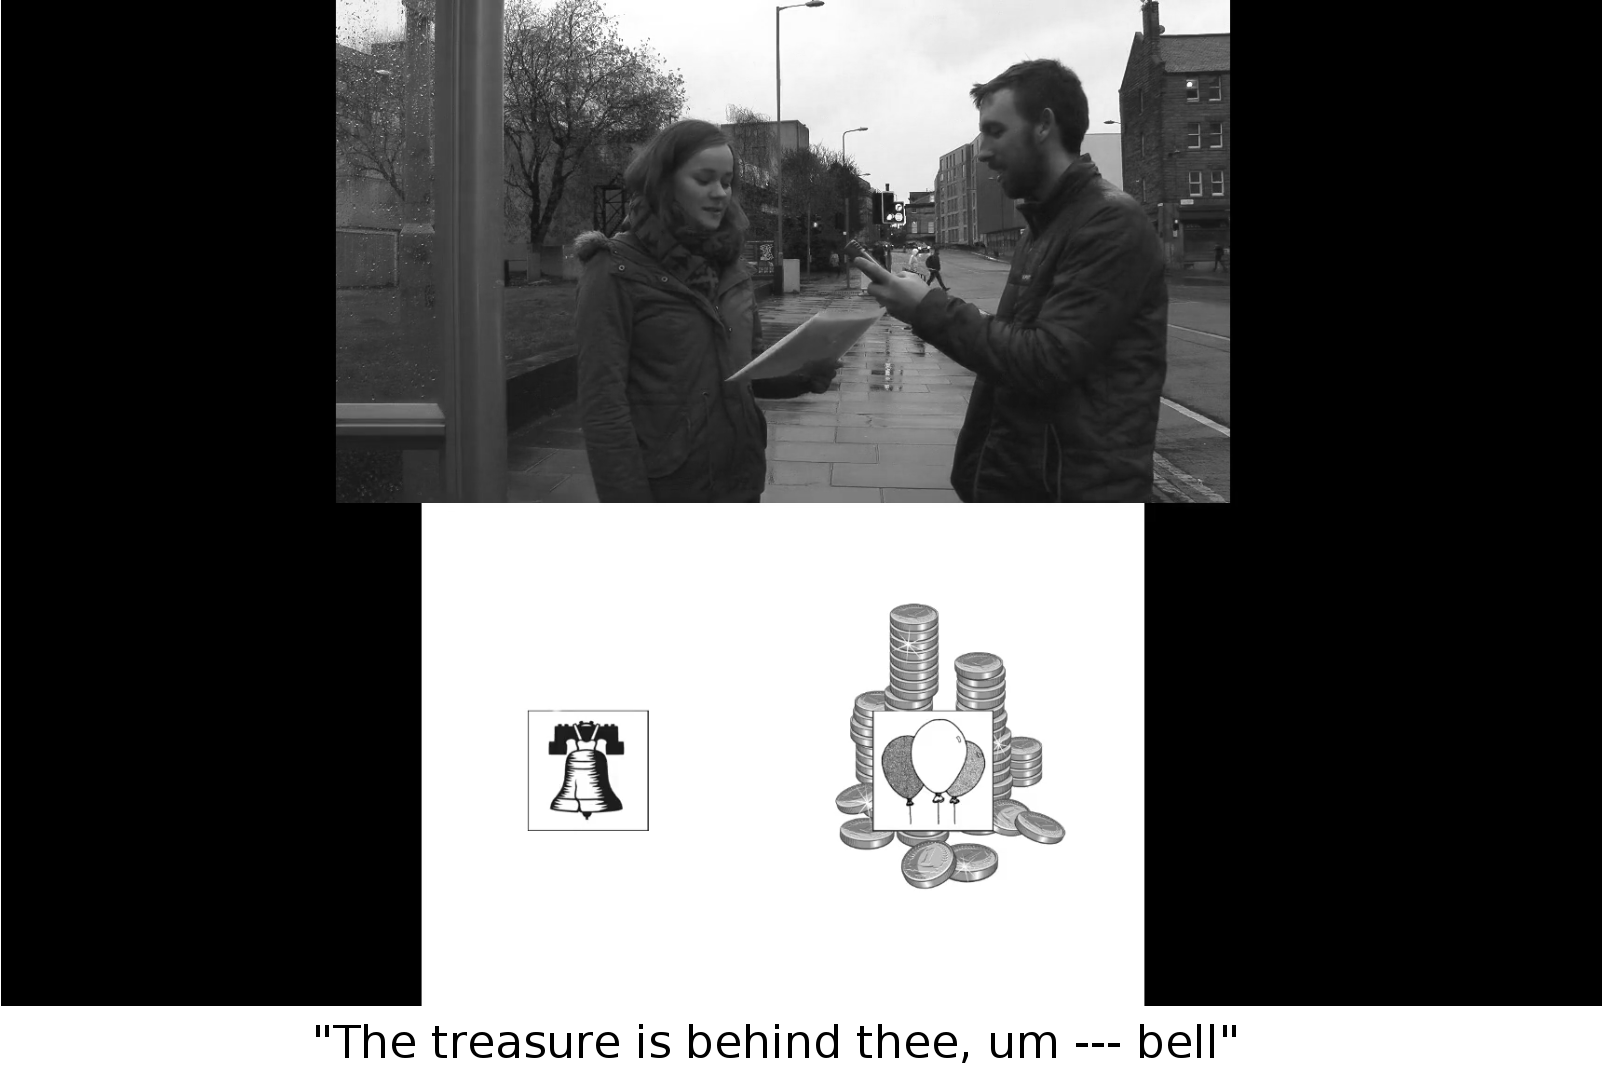
\includegraphics[scale=.2]{convincer.png}
  \caption{Screenshot of video presented to participants as an example of speaker producing utterances in a noisy environment. The screenshot shows an example of speaker producing a disfluent and dishonest utterance.}
  \label{fig:vid}
\end{figure}


To ensure that analysis could be run only on data from participants for whom the cover story held, a post-test questionnaire assessed whether participants believed that the utterances were produced outdoors, as claimed.
Once they had been debriefed about the true nature of the experiment, participants were asked again whether it had occurred to them during the experiment that the recordings might not have been produced outside in the street.

\subsection{Procedure}
Stimuli were displayed on a 21~in.\@ CRT monitor, placed 850~mm from an Eyelink~1000 Tower-mounted eye-tracker which tracked eye movements at 500~Hz (right eye only). 
Audio was presented in stereo from speakers on either side of the monitor. 
Mouse coordinates were sampled at 50~Hz. 
The experiment was presented using OpenSesame version~3.0 \citep{Mathot2012}.


%\subsubsection{trial structure}
Participants were told they would see a series of pairs of objects, and that treasure was concealed behind one of the objects in each pair.
For each trial, they would hear a speaker indicating the location of the treasure; but the speaker would be lying half of the time.
Their task was to click on the object that they believed the treasure was behind, and thus accrue treasure over the course of the experiment.

Once participants had read the instructions, the eye-tracker was calibrated.
Recalibration occurred between trials where necessary.
Each trial began with a drift correction using a central fixation point, that changed from gray to red (for 500~ms) upon successful fixation. 
Following the red fixation point, two images (referent and distractor) were presented, horizontally to the left and right of the midpoint of the screen, and the ambient traffic audio began.
Referents were presented equally often on each side.
1500~ms after the stimuli had appeared, a mouse pointer was made visible at the center of the screen, and the playback of the utterance began.
Participants used the mouse to click on one of the two objects.
Once this had happened, the stimuli disappeared and were replaced by a gray fixation dot, signifying the beginning of the next trial. 
Trials timed out after 5000~ms from utterance onset.


%\subsubsection{bonus rounds}
To maintain motivation throughout the study, participants were told that there were a number of ``hidden bonus rounds'' which offered more treasure. 
Following 25\% of the filler trials, a ``bonus round'' message appeared before progressing to the next trial.
This informed participants that they had successfully located bonus treasure (regardless of the object chosen).
Participants were also told that the top scorers would be able to enter their names on a high-score table, which was shown at the beginning of the experiment. 

Participants completed five practice trials (one of which was presented as a bonus round) prior to the main experiment. 
Eye movements, mouse coordinates and object clicked (referent or distractor) were recorded for each experimental trial.


\section{Results}
\subsection{Exclusion criteria}
Thirty-seven participants took part in the experiment, for a planned design size of~24.
Participants were recruited from the University of Edinburgh community, and participated in return for a payment of \pounds{}4.
Twelve participants were excluded on the basis that they indicated either in the post-test questionnaire~(10) or verbally~(2) that they did not believe the cover story.
One further participant was excluded because they had previously taken part in similar study.


\subsection{Analysis}
Analysis was carried out in R version~3.3.0 \citep{rbase}, using the lme4 package \citep{lme4}. 
Trials in which participants did not click on either the referent or distractor (0.01\%) were excluded from all analyses. 

Analyses for both eye and mouse movements were conducted over a time window of 800~ms from the onset of the referent name, matching the analyses in \citet{Loy2016}.
This window exceeds the duration of the longest critical referent name (776~ms) and is consistent with evidence that eye movements reflect the establishment of reference around 400-800~ms after noun onset \citep{Eberhard1995}.
Eye fixation data was averaged into 20~ms bins (of 10 samples) prior to analysis.
For each bin, we calculated the proportions of time spent fixating referent or the distractor, resulting in a measure of the proportions of fixations on either object over time.

The position of the mouse was sampled every 20~ms, corresponding to one bin of eye-tracking data.
Using the $X$ coordinates only, we calculated the number of screen pixels moved and the direction of movement (towards referent or distractor).
The cumulative distance traveled towards each object was calculated for each bin, and divided by the total distance moved, regardless of direction.
The resulting measure was the proportion of total distance traveled towards either object over time.
Trials for which the total mouse distance traveled post referent-onset was less than one third of the distance from the screen center to the near edge of an object were excluded (0.03\% of trials). 
Movements beyond the outer edge of either object were considered to be `overshooting' and were not included in calculations (4\% of samples).

We used an empirical logit transform to measure relative biases in eye and mouse movements \citep{Barr2008}.
Eye movement biases were calculated from the proportions of referent to distractor fixations;
mouse movement biases were calculated analogously.
A value of zero in either measure indicates no bias towards either object, and positive and negative values indicate a bias towards the referent and distractor respectively.
Linear mixed effects models of eye and mouse movements included fixed effects of time ($Z$-scored), delivery (fluent or disfluent) and speaker distraction (absent or present), and all interactions.
Random intercepts and slopes for time, delivery and distraction were included by subject and by referent.
Following \citet{baayen2008analyzing}, we considered effects in these models to be significant where $|t|>2$.

The object clicked (referent or distractor) was modeled using mixed effects logistic regression.
This model included  fixed effects of delivery (fluent or disfluent) and speaker distraction (absent or present), and all interactions, with random intercepts and slopes for delivery and distraction by subject and by referent.

\subsection{Object click}
Responses show the same overall tendency to interpret an utterance as truthful as was found by \citet{Loy2016}, with 57\% of trials resulting in a click on the referent and only 43\% on the distractor.
Table \ref{table:objctclck} shows the percentage of mouse-clicks on each object by condition.
Analyses showed that participants were less likely to click on the referent following a disfluent utterance than a fluent one ($\beta = -2.24$; $\SE = 0.67$; $p<.001$). 
%MC note "proper" way to typeset stats (includes real spaces etc.)
This is in keeping with the literature \citep{depaulo2003cues,Zuckerman1981}:
Manner of delivery influences participants' global interpretations of the speaker's truthfulness. 
The presence of a plausible speaker distraction was not found to affect responses; neither was the interaction between delivery and distraction. 
The bias toward interpreting disfluency as a sign of dishonesty appeared to be explicit for 19~out of~24 participants, as indicated in the post-test questionnaire. 



\begin{table}[ht]
\centering
\caption{Mouse clicks on each object by condition.}
\label{table:objctclck}
\begin{tabular}{rrrrrr}
  \hline
& \textbf{Delivery} & Disfluent & Disfluent & Fluent & Fluent \\ 
& \textbf{Speaker-distraction} & Absent & Present & Absent & Present \\
  \hline
Distractor & &  62\% &  62\% &  23\% &  24\% \\ 
  Referent & &  38\% &  38\% &  77\% &  76\% \\ 
   \hline
\end{tabular}
\end{table}

%%%MC general things: (1) in the eye movement graphs, the keys are in a very weird order...? Why describe the effects markers halfway through the list of conditions? Why is there a solid circle for |t|>2 that never appears? (2) in the mouse graphs, there are no equivalent effects markers...?

\subsection{Eye movements}
Figures \ref{fig:flueye} and \ref{fig:diseye} show the time-courses of fixations to referents and distractors over 2000~ms from referent onset, for fluent and disfluent conditions respectively.
Analyses were conducted over a time window from referent onset to 800~ms post onset.
For fluent utterances, participants displayed an early fixation bias towards the referent, which increased over time ($\beta = 0.64$; $\SE = 0.12$; $t=5.44$). 
For disfluent utterances, the fixation bias towards the referent was greatly reduced ($\beta = -0.60$; $\SE = 0.06$; $t=-10.62$), and a preference for the distractor over the referent emerged later on in the trial.
When an alternative, local cause of disfluency (the car-horn) was present prior to a disfluency, the bias towards the distractor was significantly reduced ($\beta = 0.18$; $\SE = 0.08$; $t=2.20$).
The presence of the car-horn was not found to have an effect on the tendency to fixate on the referent for fluent utterances ($t=-0.60$).


%JK Model output below
\iffalse
     AIC      BIC   logLik deviance df.resid 
 63965.5  64192.6 -31953.8  63907.5    18535 

Scaled residuals: 
     Min       1Q   Median       3Q      Max 
-2.72017 -0.81217  0.07162  0.83430  2.40949 

Random effects:
 Groups   Name               Variance Std.Dev. Corr             
 subject  (Intercept)        0.19870  0.4458                    
          time2              0.13538  0.3679   -0.64            
          deliverydisfluent  0.21796  0.4669   -0.71  0.10      
          distractionpresent 0.18110  0.4256   -0.22 -0.41  0.36
 referent (Intercept)        0.23398  0.4837                    
          time2              0.12319  0.3510   -0.69            
          deliverydisfluent  0.12515  0.3538   -0.20  0.04      
          distractionpresent 0.07829  0.2798   -0.69  0.11 -0.16
 Residual                    1.78674  1.3367                    
Number of obs: 18564, groups:  subject, 24; referent, 20

Fixed effects:
                                           Estimate Std. Error t value
(Intercept)                                -0.27445    0.14685  -1.869
time2                                       0.63704    0.11571   5.506
deliverydisfluent                           0.37085    0.13606   2.726
distractionpresent                         -0.09425    0.12098  -0.779
time2:deliverydisfluent                    -0.59827    0.05635 -10.618
time2:distractionpresent                    0.03355    0.05635   0.595
deliverydisfluent:distractionpresent        0.02966    0.08008   0.370
time2:deliverydisfluent:distractionpresent  0.17569    0.08006   2.194

Correlation of Fixed Effects:
            (Intr) time2  dlvryd dstrct tm2:dl tm2:ds dlvry:
time2       -0.680                                          
dlvrydsflnt -0.473  0.147                                   
dstrctnprsn -0.448 -0.057  0.229                            
tm2:dlvryds  0.167 -0.243 -0.361 -0.203                     
tm2:dstrctn  0.167 -0.243 -0.180 -0.406  0.500              
dlvrydsfln:  0.135 -0.149 -0.291 -0.328  0.613  0.613       
tm2:dlvryd: -0.118  0.171  0.254  0.286 -0.704 -0.704 -0.871
\fi


\begin{figure}[Ht]
  \centering
	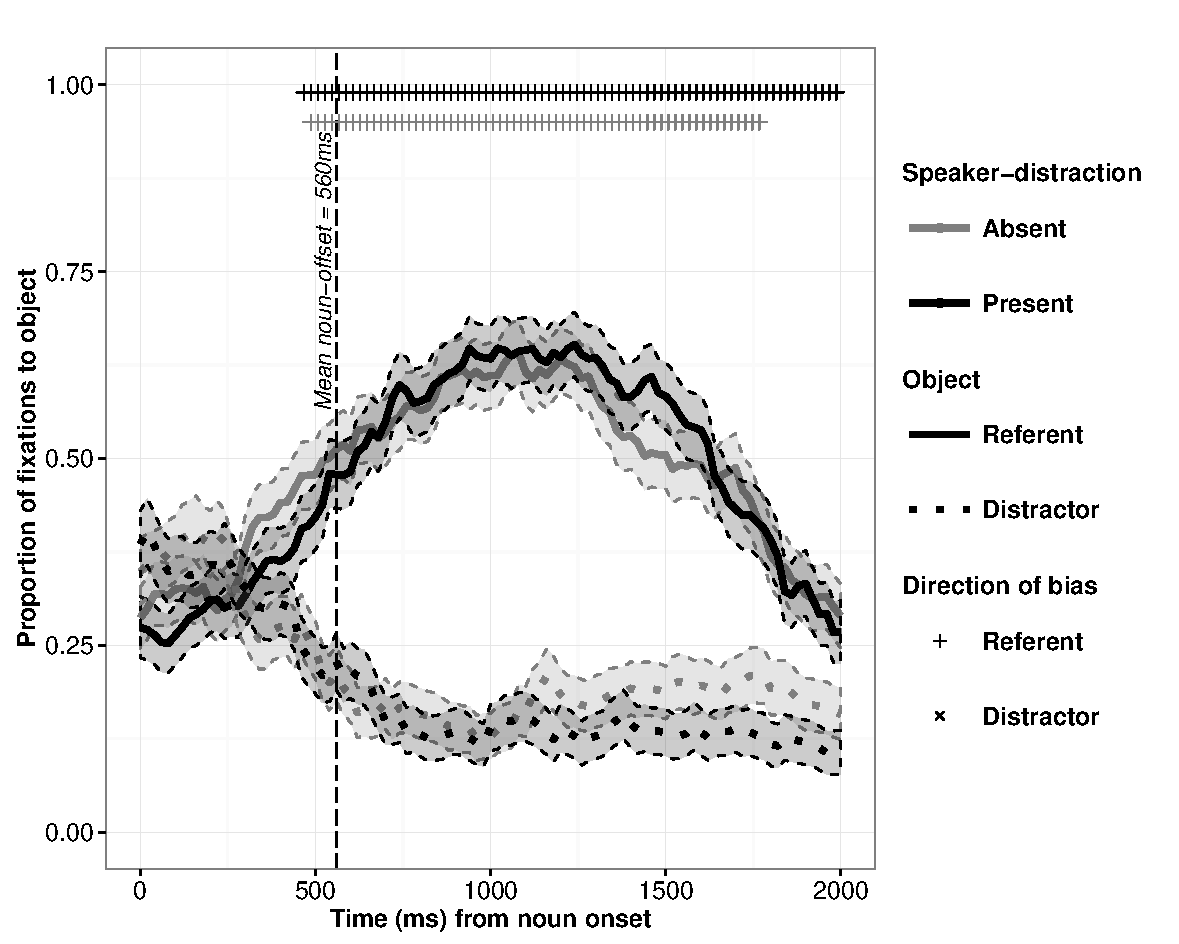
\includegraphics[width=\linewidth]{eye_fl.pdf}
  \caption{Mean proportion of fixations to either object (referent and distractor) for fluent utterances split by presence of speaker distraction, calculated out of the total sum of fixations for each 20ms time bin from referent-onset to 2000ms post-onset. Shaded areas represent $\pm 1$ standard error of the mean. Time bins in which a bias towards either the referent or distractor was evident ($|t|>2$) are highlighted with respect to condition and direction of bias (assessed by a mixed effect model estimating the empirical logit of fixations to the referent minus the empirical logit of fixations to the distractor, with by-subject and by-item random intercepts)}
  \label{fig:flueye}
\end{figure}


\begin{figure}[Ht] % might need to change placement
  \centering
	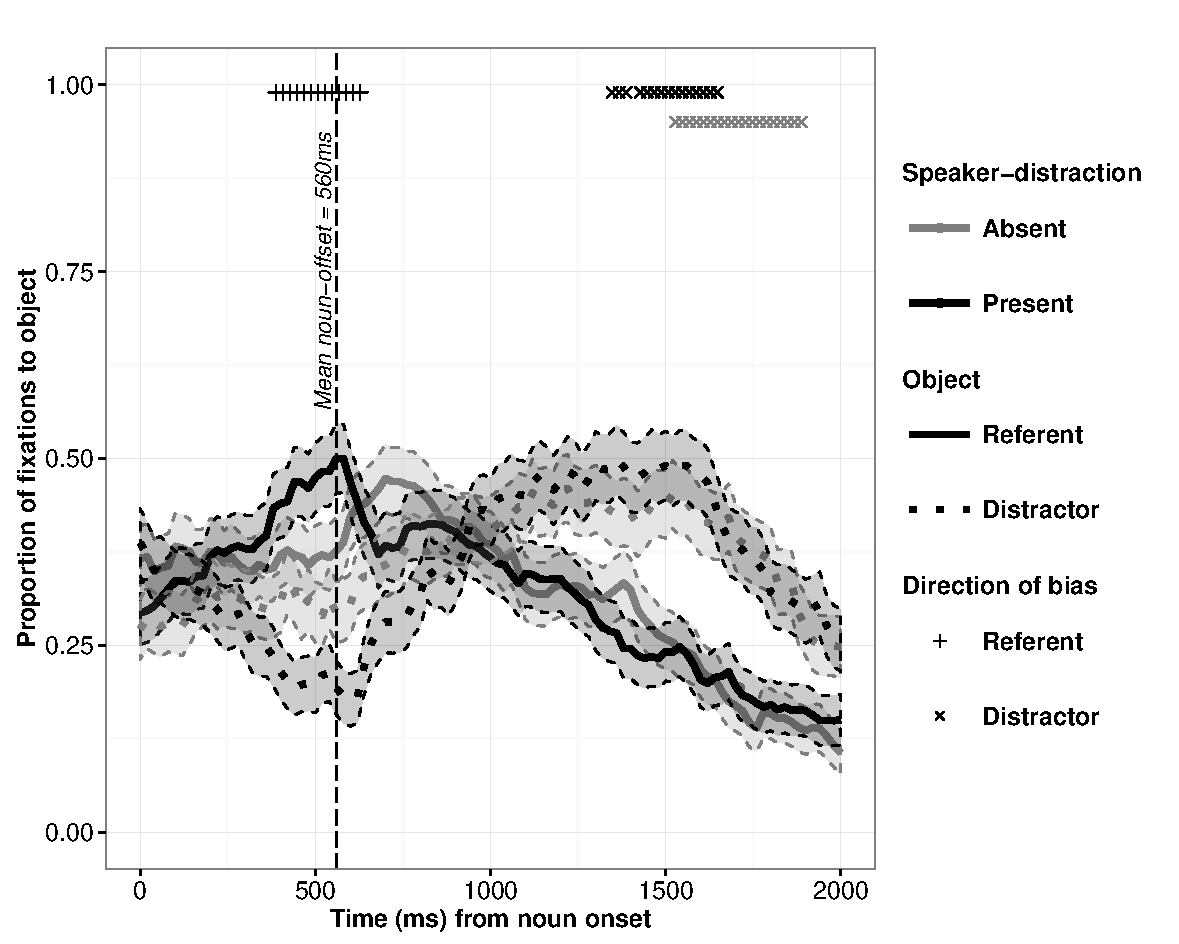
\includegraphics[width=\linewidth]{eye_disf.pdf}
  \caption{Mean proportion of fixations to either object (referent and distractor) for disfluent utterances split by presence of speaker distraction, calculated out of the total sum of fixations for each 20ms time bin from referent-onset to 2000ms post-onset. Shaded areas represent $\pm 1$ standard error of the mean. Time bins in which a bias towards either the referent or distractor was evident ($|t|>2$) are highlighted with respect to condition and direction of bias (assessed by a mixed effect model estimating the empirical logit of fixations to the referent minus the empirical logit of fixations to the distractor, with by-subject and by-item random intercepts)}
  \label{fig:diseye}
\end{figure}

\subsection{Mouse movements}
Figures \ref{fig:mflu} and \ref{fig:mdis} show the time-courses of proportionate mouse movements towards referents and distractors over 2000~ms from referent onset, for fluent and disfluent conditions respectively. 
Analyses of the window from referent onset to 800ms post-onset patterned broadly with the eye~tracking data. 
When presented with a fluent utterance, participants' movements to the referent over the distractor increased over time ($\beta = 0.49$; $\SE = 0.07$; $t=7.47$), although this movement was a little slower following a car-horn ($\beta = -0.14$; $\SE = 0.04$; $t=-3.59$).
Without distraction, participants moved the mouse towards the distractor when the delivery was disfluent ($\beta = -0.64$; $\SE = 0.04$; $t=-16.71$). 
When the car-horn was present prior to a disfluency, this tendency was greatly attenuated ($\beta = 0.37$; $\SE = 0.05$; $t=6.73$). 
%IMPORTANT %JK -- I had misread and looked at the initial effect of the car-horn, and not it's effect over time. annoying as it means eye and mouse don't pattern completely. 
%%MC moved dodgy effect into centre of paragraph.  Actually not too bad.

%JK model below
\iffalse
     AIC      BIC   logLik deviance df.resid 
 47086.7  47312.6 -23514.4  47028.7    17827 

Scaled residuals: 
    Min      1Q  Median      3Q     Max 
-3.1226 -0.4097 -0.0386  0.4392  3.4683 

Random effects:
 Groups   Name               Variance Std.Dev. Corr             
 subject  (Intercept)        0.02688  0.1639                    
          time3              0.03029  0.1741    0.03            
          deliverydisfluent  0.06708  0.2590   -0.48  0.21      
          distractionpresent 0.09474  0.3078   -0.78 -0.39  0.03
 referent (Intercept)        0.06437  0.2537                    
          time3              0.04759  0.2181   -0.63            
          deliverydisfluent  0.11471  0.3387   -0.58  0.28      
          distractionpresent 0.05744  0.2397   -0.34 -0.19 -0.21
 Residual                    0.79566  0.8920                    
Number of obs: 17856, groups:  subject, 24; referent, 20

Fixed effects:
                                           Estimate Std. Error t value
(Intercept)                                -0.19960    0.07109  -2.808
time3                                       0.49324    0.06606   7.467
deliverydisfluent                           0.35740    0.10000   3.574
distractionpresent                          0.04868    0.09103   0.535
time3:deliverydisfluent                    -0.64220    0.03843 -16.712
time3:distractionpresent                   -0.13761    0.03832  -3.591
deliverydisfluent:distractionpresent       -0.10639    0.05448  -1.953
time3:deliverydisfluent:distractionpresent  0.36643    0.05444   6.731

Correlation of Fixed Effects:
            (Intr) time3  dlvryd dstrct tm3:dl tm3:ds dlvry:
time3       -0.495                                          
dlvrydsflnt -0.573  0.311                                   
dstrctnprsn -0.523 -0.121 -0.006                            
tm3:dlvryds  0.229 -0.284 -0.333 -0.179                     
tm3:dstrctn  0.230 -0.285 -0.163 -0.366  0.490              
dlvrydsfln:  0.185 -0.174 -0.269 -0.295  0.612  0.612       
tm3:dlvryd: -0.162  0.201  0.235  0.258 -0.706 -0.703 -0.870
\fi



\begin{figure}[Ht]
  \centering
	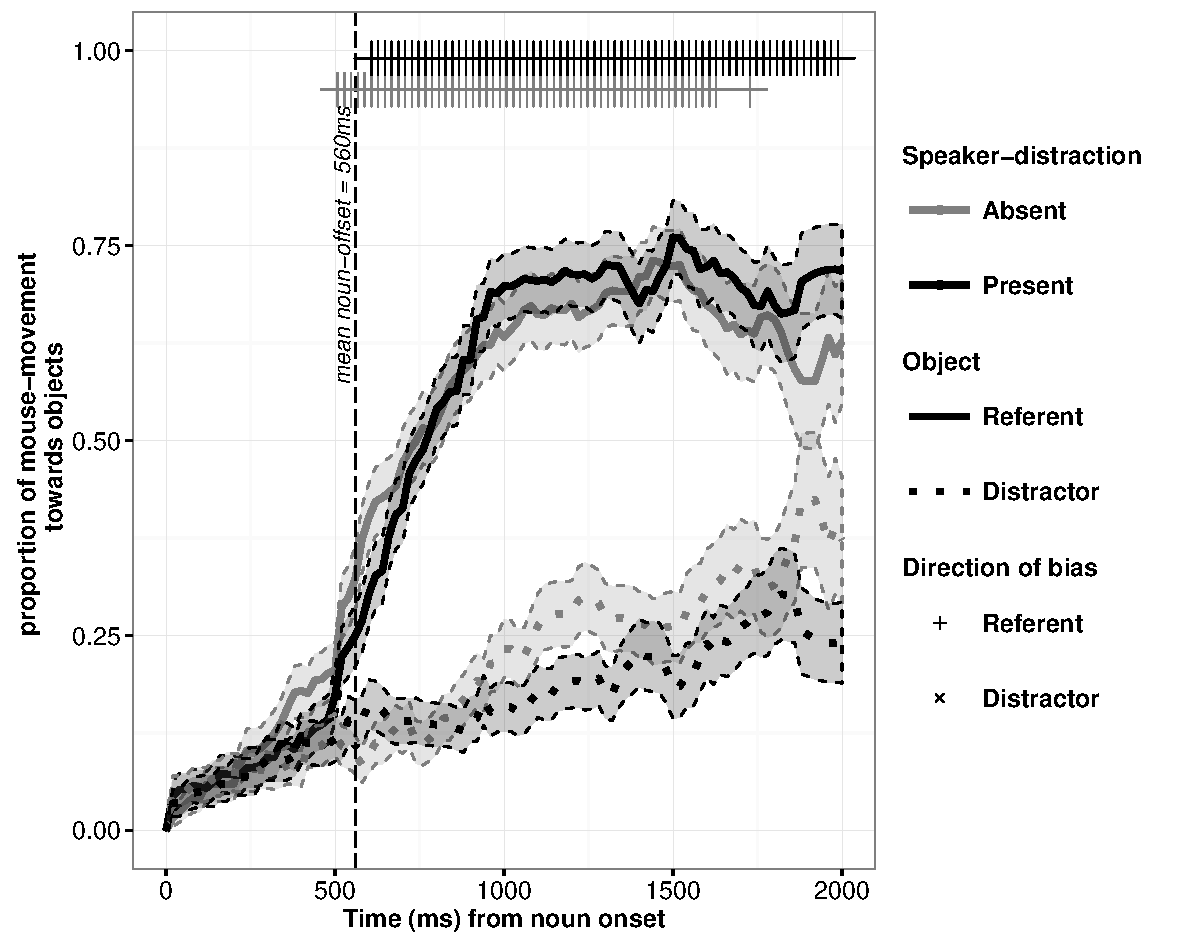
\includegraphics[width=\linewidth]{mouse_fl.pdf}
  \caption{Mean proportion of cumulative distance traveled toward each object (referent or distractor) in fluent conditions split by presence of speaker distraction, from referent onset to 2000ms post-onset. Proportions calculated out of total cumulative distance moved the mouse from referent-onset until that time bin. Shaded areas represent $\pm 1$ standard error of the mean. Time bins in which a bias towards either the referent or distractor was evident ($|t|>2$) are highlighted with respect to condition and direction of bias (assessed by a mixed effect model estimating the empirical logit of movements to the referent minus the empirical logit of movements to the distractor, with by-subject and by-item random intercepts)}
  \label{fig:mflu}
\end{figure}


\begin{figure}[Ht]
  \centering
	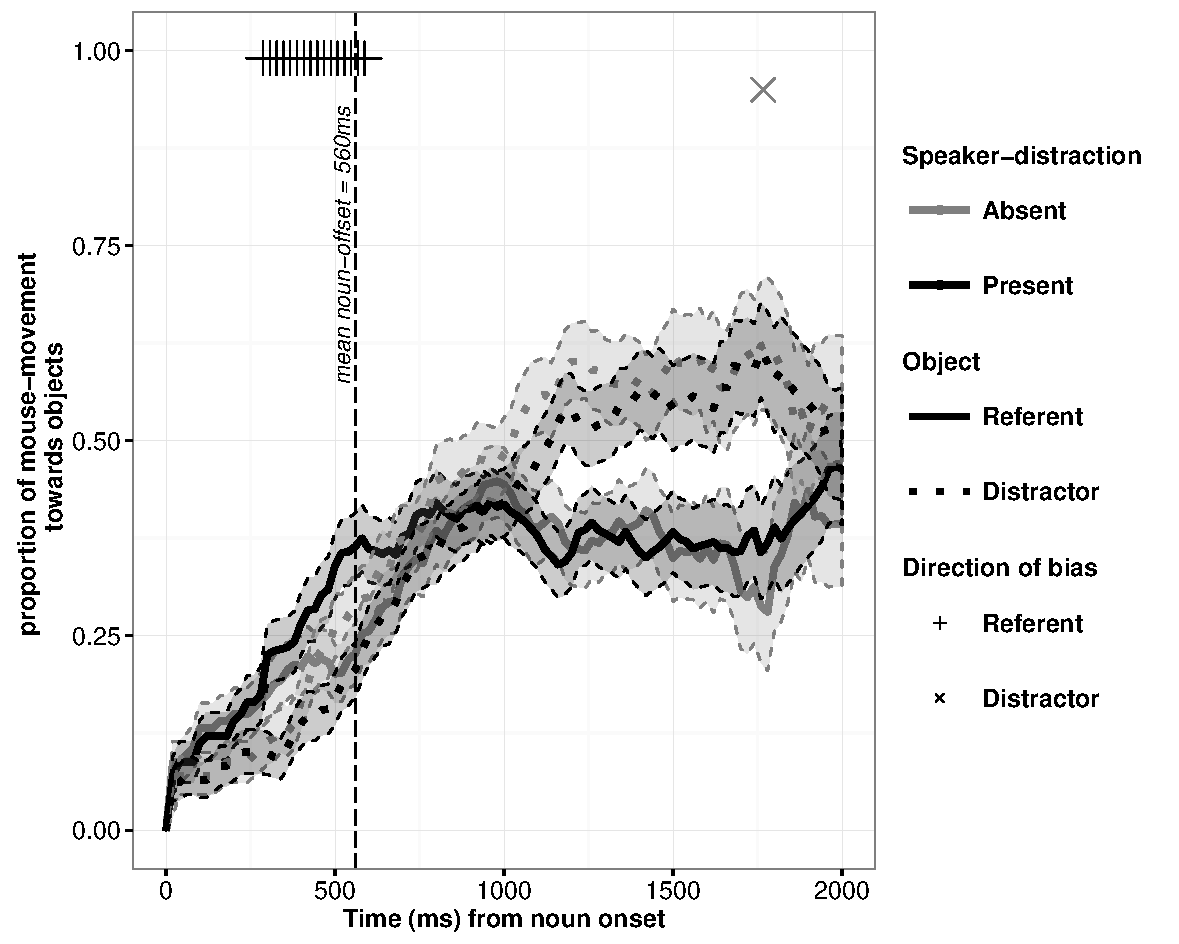
\includegraphics[width=\linewidth]{mouse_disf.pdf}
  \caption{Mean proportion of cumulative distance traveled toward each object (referent or distractor) in disfluent conditions split by presence of speaker distraction, from referent onset to 2000ms post-onset. Proportions calculated out of total cumulative distance moved the mouse from referent-onset until that time bin. Shaded areas represent $\pm 1$ standard error of the mean. Time bins in which a bias towards either the referent or distractor was evident ($|t|>2$) are highlighted with respect to condition and direction of bias (assessed by a mixed effect model estimating the empirical logit of movements to the referent minus the empirical logit of movements to the distractor, with by-subject and by-item random intercepts)}
  \label{fig:mdis}
\end{figure}


\section{Discussion}
Listeners' pragmatic judgments about a speaker's honesty were affected by manner of delivery.
In keeping with the literature on deception perception, participants associated speaker disfluency with lying \citep{Zuckerman1981,depaulo2003cues}. 
As also shown by \citet{Loy2016}, listeners made these judgments quickly.
Both eye- and mouse-tracking evidence showed that biases emerged early, with listeners committed to a pragmatic interpretation of the speaker's honesty almost as quickly as the intended referent could be identified.
These effects were shown to be robust against the presentation of speech in a noisy environment, in which there are potential distractions for the listener.

%%%MC note linking phrase---always handy :)
Importantly, listeners were not neutral with regard to the available distractions.
Where a background noise (a car-horn) was a plausible cause of the speaker's disfluency, participants showed an initial tendency both to fixate and to move the mouse pointer towards the referent, only later fixating on and eventually clicking on the distractor.
%%%MC note rhetorical emphasis that this is shown in two measures
Note that this finding suggests that listeners are sensitive to momentary changes to the context in which speech occurs.
In this respect, it differs from \citegen{Arnold2007} earlier finding that (constant) knowledge about the speaker can affect the ways in which listeners respond to disfluency.
At face value, the finding may be taken to suggest that listeners in the present study are modeling the speaker's production system in enough detail to be able to attribute a particular cause to a given disfluency.

%%MC some argumentation here is completely new.  It's actually alternative (1) which worries me the most, which is why I've tried to dismiss it out-of-hand.
%%JK possibly harder to dismiss it, with the mouse-movements as they are..
There are, however, two potential alternative accounts of this finding.
The first is that it was in fact the participants who were distracted by the car-horns, and that the findings reflect their initial lack of attention to the speaker's disfluency, rather than any attempt to model the cause of that disfluency.
There is possible evidence for this in the fact that the car-horn was found to influence participants' mouse movements during fluent utterances. 
With attention to any disfluency attenuated, there might be an initial bias to interpret utterances as honest. 
%JK but then the car-horn in the fluent utterances makes people move more towards the distractor?
The account becomes difficult to sustain when we take the entire pattern of results into account, though, as the `unattended' disfluencies clearly influence the eventual pragmatic interpretations of the speaker's utterances.

The second alternative account is that participants' pragmatic judgments relied on a heuristic association between disfluency and dishonesty.
If the heuristic were to take into account any loud noises which preceded a disfluency, then participants might be expected to behave very much like the ones in the present experiment.
This interpretation would leave us with two questions to answer, though.
The first concerns the specificity of the heuristic.
Might it be sensitive to car-horns, but not to dog barks, for example?
Would it be contextually sensitive?
Would listeners discern between the car-horn in the present experiment, which was contextually linked to the recording of the speaker, and a similarly loud car-horn which happened to sound `outside the testing room'?
The second question is that of how the heuristic is created in the first place.
One possibility is that it is trained on co-occurrences (that is, participants have previously observed car-horns to be associated with disfluency, and disfluency with lying).
Unless any loud noise acted as a cause of disfluency, such a system would quickly run into a data scarcity problem \citep[see][for a similar argument concerning parsing]{Mitchell:ea:95}.
Another possibility is that the heuristic is based upon introspection, or the listener's own understanding of what they would do as a speaker in given circumstances.
To the extent that the latter is true, a heuristic is simply a form of speaker modeling (perhaps with differing implementational details).

The evidence therefore remains consistent with the view that listeners are able to reason dynamically about the most likely explanation of disfluency, and, as the speech unfolds, make attributions about why a particular speaker in a particular context has been disfluent.
This is in line with the speaker modeling account found in lying research, suggesting that listeners detect deception by reasoning about cues relating to the cognitive load of the speaker \citep{Zuckerman1981,depaulo2003cues}.
From this perspective, the findings here---that an alternative cause of disfluency modulates listeners' attributions of deception to disfluency---suggest that speaker modeling affects the early stages of comprehension.

%%%%% MC GOT AS FAR AS HERE

Of note is the fact that \citet[][Experiment~3]{Arnold2007} did not find that distracting noises affected listeners' predictions about what speakers were likely to mention following a disfluency.
There are a couple of possible reasons for this difference.
Trivially, differences between experiments---the construction of utterances, for example---might simply mean that in the present experiment disfluency appeared more believably caused by distraction.
Alternatively, it might be that the requirement to infer a pragmatic meaning in the lying paradigm renders listeners more likely to model the causes of disfluency.
In particular, the treasure hunting game requires participants to reason about the speaker, and thus may encourage reasoning about the detail of the speaker's utterances.
It may be that listeners can take context into account when it matters, but may not always do so, perhaps because for other effects of disfluency there are often no lasting consequences.

The fact that participants in this experiment are led to reason about the speaker might also go some way to explaining the overall bias to interpret disfluency as a cue to deception.
Although the car-horn had a clear influence on the evaluation of disfluency, this effect was only temporary, as shown by participants' clicks on the referent or distractor objects.
At the end of each utterance, listeners' interpretations were open to explicit reasoning; and initial interpretations appear to have been largely overridden.
The fact that 19~out of~24 participants explicitly linked disfluency with deception in the post-test questionnaire supports this view, and opens up the possibility that in a less game-like environment, the contribution of environmental factors to a speaker model would be larger.
%JK 'explicit' or 'conscious'?

The availability of an alternative, local cause of disfluency influenced the initial stages of participants' judgments about a speaker's honesty. 
The current study shows that, in situations which require reasoning about a speaker's honesty, listeners are sensitive to disfluencies and the context in which they occur.
This sensitivity is shown simultaneously in eye movements and mouse movements, building on support for mouse tracking as an alternative way of tracking cognitive processes \citep[e.g.,][]{farmer07}.
%JK insert mouse~tracking bit here? even though doesn't fully pattern? I mean, it does for disfluent, just not fluent..
The findings are in line with suggestions in the deception literature that listeners associate disfluency with lying because of a speaker model which links lying to cognitive effort, and effort to disfluency.
Moreover, they build on earlier work by \citet{Arnold2007}, showing that, in cases where the pragmatic meaning of an utterance is at stake, listeners are able to take momentary contextual causes of disfluency into account.
Above all, the present study emphasizes that understanding a speaker's pragmatic intentions is a contextually rich, and very fast, process. 



\bibliography{e2}

\end{document}
%%% Local Variables:
%%% mode: latex
%%% TeX-master: t
%%% End:
